\section{Method}
\label{sec:method}



\begin{figure*}[t]
    \centering
    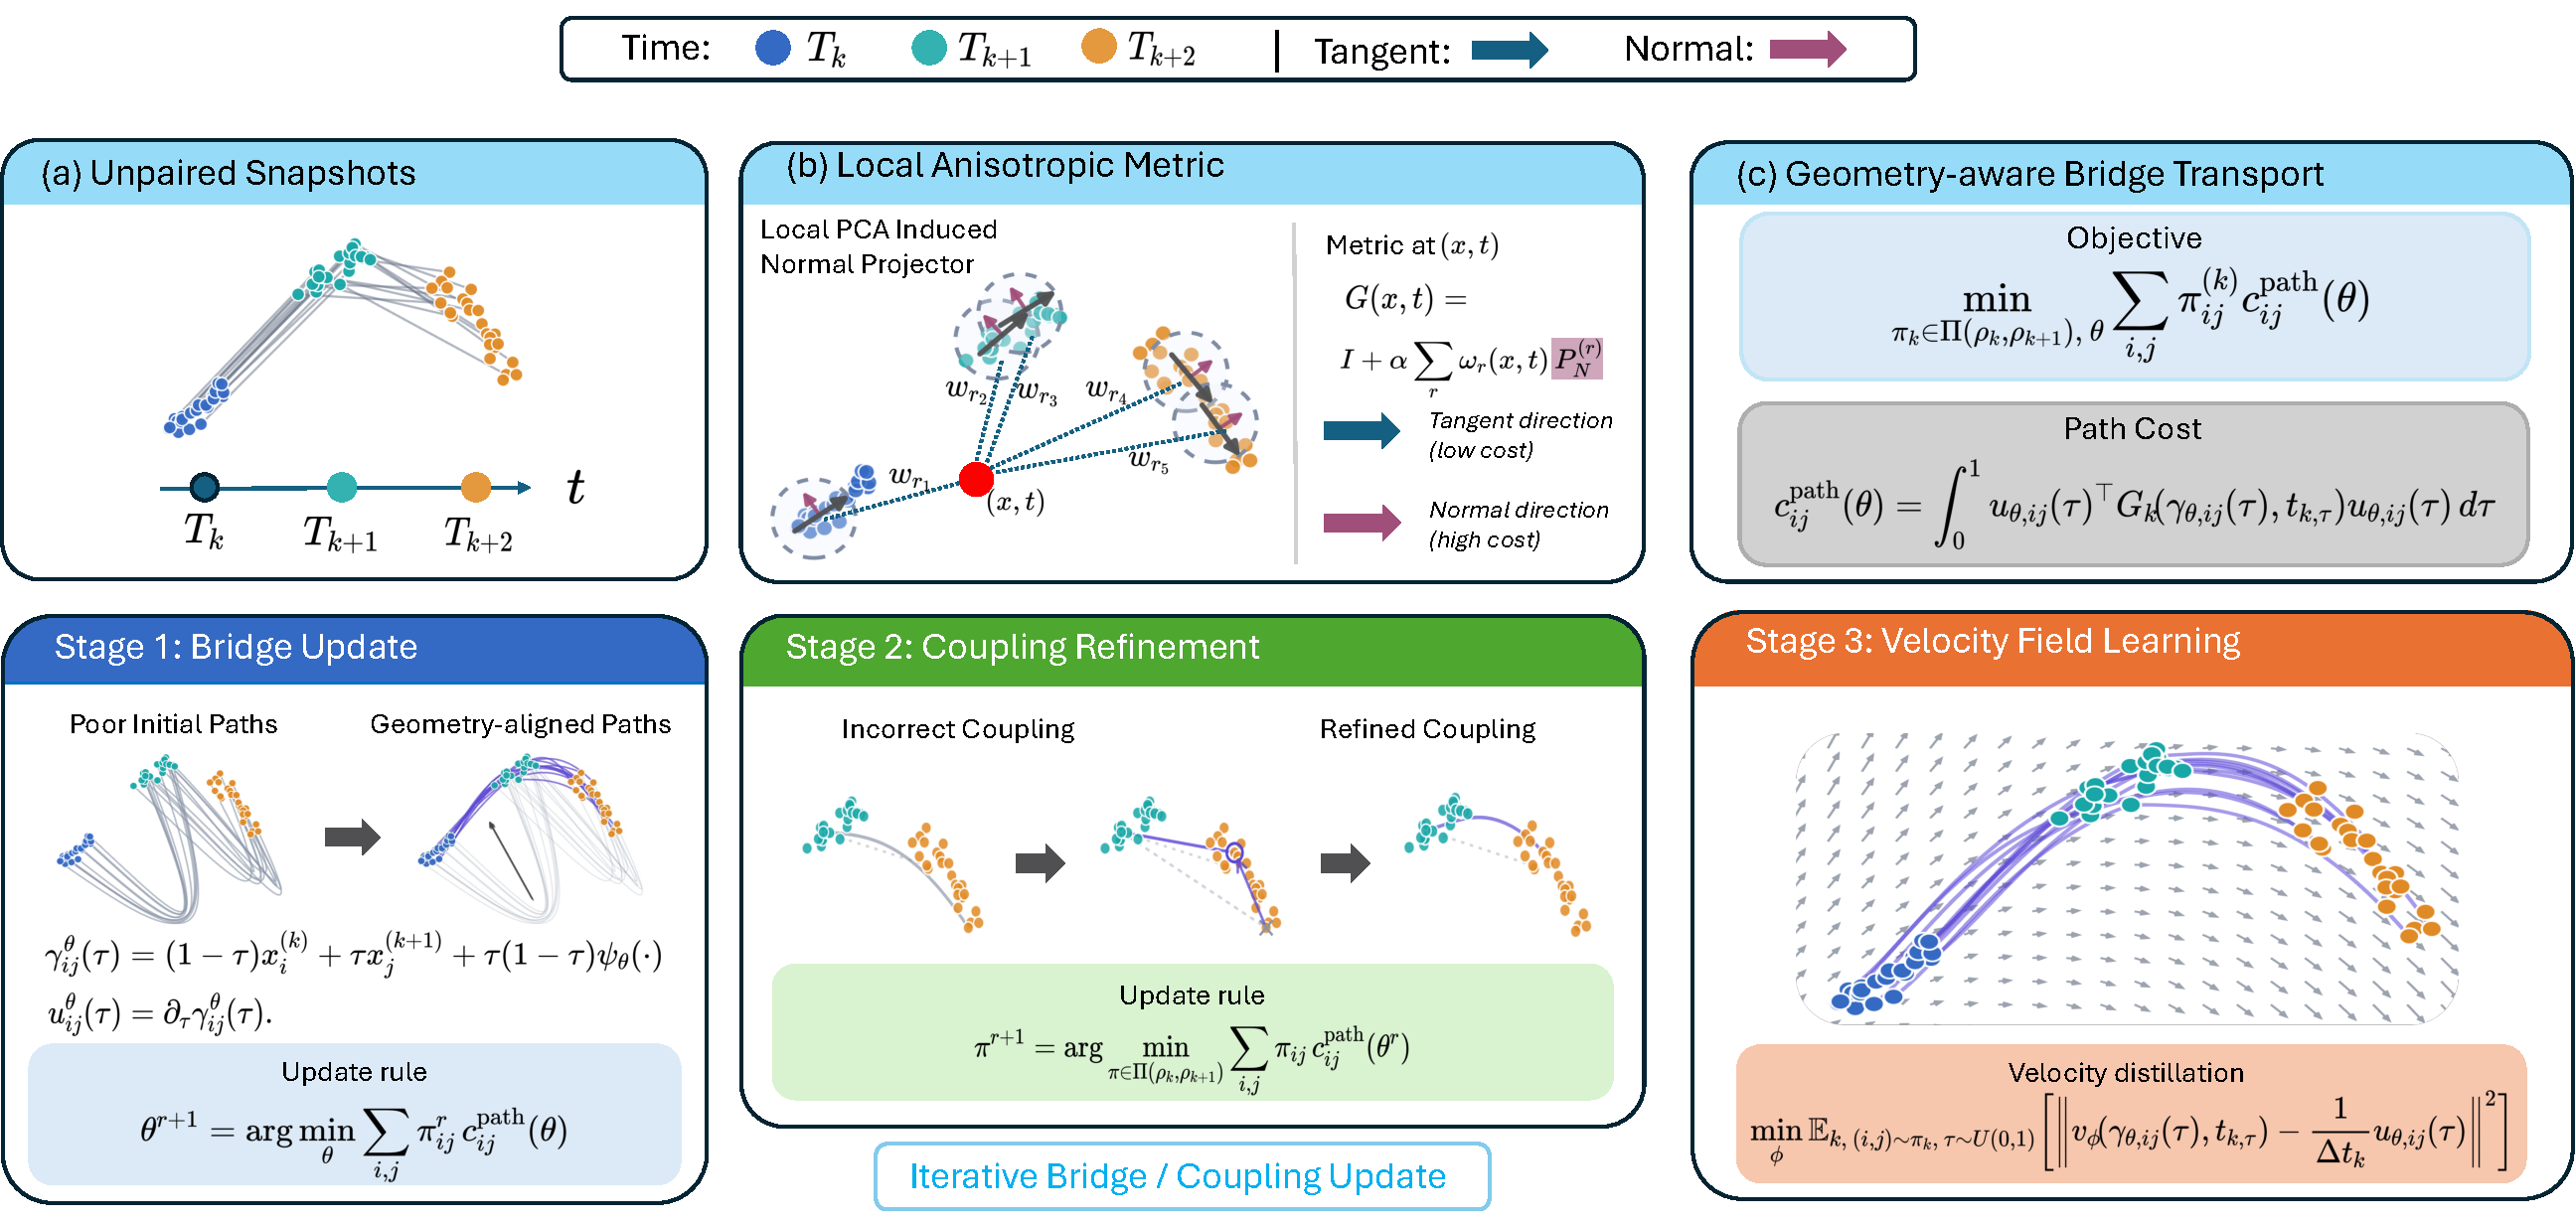
\includegraphics[width=0.92\textwidth]{figures/fig1.pdf} % PAGECUT: was width=\textwidth (NeurIPS layout)
    \caption{
    \textbf{Overview of PACE.}
    PACE uses local PCA to construct an anisotropic metric \(G_k(x,t)=I+\alpha C_N^{(k)}(x,t)\), trains endpoint-preserving neural bridges under the corresponding path-action cost, iteratively refines cross-time couplings, and distills the learned bridge dynamics into a global velocity field.
    } % PAGECUT: dropped redundant tail "for trajectory inference from unpaired snapshots" (original caption preserved in git history / arXiv source)
    \label{fig:pace_overview}
\end{figure*}


\subsection{Problem formulation}
\label{sec:problem-formulation}

We observe single-cell point clouds at anchor times
\(\{t_k\}_{k=0}^K\), with \(t_0=0\),
\[
\mathcal{X}^{(k)}
=
\{x_i^{(k)}\}_{i=1}^{N_k}
\sim \hat\rho_k
\subset \mathbb{R}^d,
\qquad
k=0,1,\dots,K.
\]
Here \(d\) denotes the representation dimension.
Our goal is to infer trajectories and a velocity field transporting \(\hat\rho_k\) to \(\hat\rho_{k+1}\) between adjacent times.
Once learned, the velocity field can be integrated from \(x_{t_0}\sim\hat\rho_0\) to generate trajectories over the time course.

\begin{proposition}[Ill-posedness from snapshots alone]
\label{prop:illposed}
Given only the point clouds \(\{\mathcal{X}^{(k)}\}_{k=0}^K\), the reconstruction of cross-time couplings and intermediate trajectories is non-unique.
\end{proposition}

Indeed, for a single interval \([t_k,t_{k+1}]\), many couplings \(\pi_k\in\Pi(\hat\rho_k,\hat\rho_{k+1})\) share the same endpoint marginals. For any such coupling, each coupled endpoint pair can also be connected by infinitely many smooth paths. Thus, the observed snapshots determine neither a unique correspondence nor a unique intermediate trajectory. This observation motivates PACE to frame trajectory inference as a variational problem over couplings and paths, selected by a geometry-aware path action. The proof of Proposition~\ref{prop:illposed} is given in Appendix~\ref{app:illposed}.

\subsection{Geometry-aware bridge transport}
\label{sec:variational-principle}

To address the ill-posedness in Proposition~\ref{prop:illposed}, PACE formulates trajectory reconstruction as selecting both a cross-time coupling and a family of continuous paths, chosen by minimizing a geometry-aware action.
Given a time- and state-dependent metric tensor \(G_k(x,t)\) (constructed in \S\ref{sec:metric}), the cost of a path \(\gamma\), or 
"path action", between endpoints \((x,y)\) is
\begin{equation}
\label{eq:pace-path-action}
\mathcal{A}_{G_k}[\gamma]
=
\int_0^1
\dot\gamma(\tau)^\top
G_k\!\bigl(\gamma(\tau),\,t_{k,\tau}\bigr)
\dot\gamma(\tau)
\,d\tau,
\qquad
\gamma(0)=x,\;\gamma(1)=y,
\end{equation}
where \(\tau\in[0,1]\) is local interpolation time and the physical time is \(t_{k,\tau}=t_k+\tau(t_{k+1}-t_k)\).
The path action first defines the geometry-aware endpoint cost, and the ideal PACE bridge problem then transports mass using this induced cost:
\begin{empheq}[box=\eqbox]{equation}
\label{eq:ideal-pace-bridge}
\begin{aligned}
c_{G_k}(x,y)
&=
\inf_{\substack{\gamma(0)=x\\ \gamma(1)=y}}
\mathcal{A}_{G_k}[\gamma],&
\pi_k^\star
\in
\arg\min_{\pi_k\in\Pi(\hat\rho_k,\hat\rho_{k+1})}
\int
c_{G_k}(x,y)
\,d\pi_k(x,y).
\end{aligned}
\end{empheq}
Here \(c_{G_k}(x,y)\) is not a fixed Euclidean endpoint distance; it is the minimum action required to move from \(x\) to \(y\) under the metric \(G_k\).

This formulation makes explicit how PACE differs from standard OT.
If \(G_k(x,t)\equiv I\), then Eq.~\eqref{eq:pace-path-action} reduces to the Euclidean kinetic energy.
For any fixed endpoint pair \((x,y)\), the minimum-action path is the straight constant-speed interpolant, and the induced cost becomes
$
c_{G_k}(x,y)=\|y-x\|^2.
$
In this special case, Eq.~\eqref{eq:ideal-pace-bridge} reduces to standard quadratic-cost OT between \(\hat\rho_k\) and \(\hat\rho_{k+1}\).

PACE departs from this Euclidean case by using a state- and time-dependent anisotropic metric \(G_k(x,t)\).
The induced cost \(c_{G_k}(x,y)\) is no longer determined only by endpoint distance; it depends on the entire path and on how the \emph{path velocity} aligns with local developmental geometry.
As a result, the minimum-action cost generally has no closed-form solution and cannot be reduced to a fixed Euclidean endpoint cost.
The next section defines the spatiotemporal metric \(G_k(x,t)\), and \S~\ref{sec:alternating} describes how PACE approximates this 
problem with neural bridges and alternating coupling updates.




\paragraph{Finite-dimensional approximation.}
Problem~\eqref{eq:ideal-pace-bridge} is an ideal infinite-dimensional formulation.
PACE makes it tractable through two approximations (\S\ref{sec:alternating}):
(i) the path family is parameterized by neural bridges \(\gamma_\theta\) that satisfy endpoint constraints by construction;
(ii) the action integral is approximated on a finite time grid.
These yield a finite-dimensional alternating optimization over bridge parameters and correspondence variables.


\subsection{Time-dependent spatiotemporal tangent metric}
\label{sec:metric}

The metric should encode a simple prior: admissible motion should follow directions locally supported by the observed geometry, rather than cut across the cell-state manifold. Although local neighborhoods do not reveal the true direction of time, their dominant variation directions provide an undirected tangent approximation to the set of plausible state changes.
PACE therefore treats tangent motion as low cost and penalizes velocity components in the locally estimated normal subspace.
Because the local composition and geometry of snapshots can change across experimental time, the admissible subspaces are indexed by both state and time, yielding a time- and state-dependent metric \(G_k(x,t)\).
	        
        \paragraph{Local normal subspaces.}
        At each anchor point \(x_r\) observed at time \(t_r\), PACE estimates an anchor-wise local normal direction by finding its \(m_{\rm nn}\) nearest spatial neighbors within the same snapshot (including \(x_r\) itself), computing a Gaussian-kernel weighted covariance of the neighbor cloud, and extracting the minimum-variance principal direction \(n_r\).
        In two dimensions the normal projector is simply \(P_N^{(r)}=n_r n_r^\top\); in higher dimensions PACE adaptively selects the tangent-subspace dimension
        and builds the normal projector as the orthogonal complement (Appendix~\ref{app:adaptive-projectors}).
        
        \paragraph{Spatiotemporal metric construction.}
        For a query point \((x,t)\) in segment \(k\), PACE interpolates these anchor-wise local normal projectors across state and time using space-time Gaussian weights over all anchor points \(r\):
        \begin{equation}
            \label{eq:weights}
            \omega_r^{(k)}(x,t)
            \propto
            \exp\!\left(
            -\frac{\|x-x_r\|^2}{(h_x^{(k)})^2}
            -\frac{|t-t_r|^2}{(h_t^{(k)})^2}
            \right),
        \end{equation}
        with normalization chosen so that \(\sum_r\omega_r^{(k)}(x,t)=1\), where the bandwidths \(h_x^{(k)}\) and \(h_t^{(k)}\) are estimated adaptively for each segment (see Appendix~\ref{app:bandwidth}).
        These weights define an averaged normal projector field and the corresponding metric tensor
        \[
        C_N^{(k)}(x,t)=\sum_r \omega_r^{(k)}(x,t)P_N^{(r)}, \qquad G_k(x,t)=I+\alpha C_N^{(k)}(x,t),\qquad \alpha>0.
        \]
        The corresponding velocity cost is \(v^\top G_k(x,t)v = \|v\|^2 + \alpha\, v^\top C_N^{(k)}(x,t)\,v\). Because \(C_N^{(k)}\) is a positive-semidefinite average of local normal projectors, the second term increases the cost most strongly for velocities aligned with nearby estimated normal directions.


        
        \begin{proposition}[Normal-subspace penalizing property]
        \label{prop:metric}
        For every segment \(k\), query point \((x,t)\), and velocity \(v\in\mathbb{R}^d\),
        \begin{equation}
        \label{eq:metric-psd}
        v^\top G_k(x,t)v
        =
        \|v\|^2
        +
        \alpha v^\top C_N^{(k)}(x,t)v
        \ge
        \|v\|^2.
        \end{equation}
        Moreover, if \(C_N^{(k)}(x,t)=P_N(x,t)\) is an exact orthogonal projector onto the normal subspace \(T_{x,t}^{\perp}\), and \(v=v_T+v_N\) with \(v_T\in T_{x,t}\) and \(v_N\in T_{x,t}^{\perp}\), then
        \begin{equation}
        \label{eq:tangent-normal-cost}
        v^\top G_k(x,t)v
        =
        \|v_T\|^2
        +
        (1+\alpha)\|v_N\|^2.
        \end{equation}
        \end{proposition}
        
        Proposition~\ref{prop:metric} shows that the interpolated metric always preserves at least the Euclidean velocity cost, and that tangent motion retains its Euclidean cost while normal motion is penalized by a factor \(1+\alpha\) in the ideal projector case.
        Thus, the metric turns the qualitative principle of geometry-aligned cellular motion into an explicit action functional.

    \subsection{Finite-dimensional optimization by alternating bridge and OT coupling updates}
    \label{sec:alternating}

    PACE approximates the anisotropic bridge problem by alternating between an endpoint-conditioned bridge and a cross-time coupling. The coupling determines which endpoint pairs are used to train the bridge, while the bridge induces a path-action cost for updating the coupling. This creates a bootstrap mechanism in which more plausible couplings provide better endpoint supervision, and better bridges provide a geometry-aware approximation to the endpoint cost used for OT refinement. Since solving a separate minimum-action path problem for every candidate endpoint pair is infeasible under the state- and time-dependent metric $G_k(x,t)$, PACE amortizes path optimization with a shared endpoint-preserving neural bridge $\gamma_\theta(x,y,\tau)$. See Appendix~\ref{app:alternating-intuition} for a detailed discussion of this alternating procedure.

    \paragraph{Endpoint-preserving neural bridge.}
    For an endpoint pair \((x,y)\in\mathbb{R}^d\times\mathbb{R}^d\) and local time \(\tau\in[0,1]\), we define
    \begin{equation}
    \label{eq:bridge}
    \gamma_\theta(x,y,\tau)
    =
    (1-\tau)x+\tau y
    +
    \tau(1-\tau)\psi_\theta(x,y,\tau),
    \end{equation}
    where \(\psi_\theta:\mathbb{R}^d\times\mathbb{R}^d\times[0,1]\to\mathbb{R}^d\) is a neural network. The factor \(\tau(1-\tau)\) enforces \(\gamma_\theta(x,y,0)=x\) and \(\gamma_\theta(x,y,1)=y\), so the network only controls the interior deformation of the path~\citep{petrovic2026curly}. The bridge velocity is \(u_\theta(x,y,\tau)=\partial_\tau\gamma_\theta(x,y,\tau)\), computed by automatic differentiation. When \(\psi_\theta=0\), the bridge reduces to the straight Euclidean interpolant.


    
\paragraph{Bridge learning under fixed coupling.}
Assume that, for each adjacent snapshot pair, a coupling \(\pi_k\in\Pi(\hat\rho_k,\hat\rho_{k+1})\) is given. During the bridge update, endpoint pairs \((x_i^{(k)},x_j^{(k+1)})\sim\pi_k\) are sampled from the current coupling. We write \(t_{k,\tau}=t_k+\tau(t_{k+1}-t_k)\).

PACE trains the endpoint-preserving bridge by minimizing
\begin{equation}
\label{eq:total-loss}
\mathcal{L}_{\mathrm{bridge}}(\theta)
=
\lambda_{\mathrm{metric}}\mathcal{L}_{\mathrm{metric}}
+
\lambda_{\mathrm{reg}}\mathcal{L}_{\mathrm{reg}}.
\end{equation}
The main term $\mathcal{L}_{\mathrm{metric}}$ is the anisotropic bridge action induced by the spatiotemporal metric $G_k$.
An optional regularization term $\mathcal{L}_{\mathrm{reg}}$ penalizes large normal components and incoherent cross-segment velocities (Appendix~\ref{app:regularizers}).

The metric-action loss is
\begin{equation}
\label{eq:metric-loss}
\mathcal{L}_{\mathrm{metric}}
=
\mathbb{E}_{k,(x,y)\sim\pi_k}
\left[
\frac{1}{T}
\sum_{\ell=1}^{T}
u_\theta(x,y,\tau_\ell)^\top
G_k\!\left(
\gamma_\theta(x,y,\tau_\ell),
t_{k,\tau_\ell}
\right)
u_\theta(x,y,\tau_\ell)
\right].
\end{equation}
    
\paragraph{Coupling update under fixed bridge.}
After the bridge model has been updated under the current coupling, PACE recomputes the coupling using the full path action rather than Euclidean endpoint distance. For a candidate source-target pair \((x_i^{(k)},x_j^{(k+1)})\), the path-action cost is
\begin{equation}
\label{eq:path-cost}
c_{ij}^{\mathrm{path}}(\theta)
=
\frac{1}{M}
\sum_{m=1}^{M}
u_\theta(x_i^{(k)},x_j^{(k+1)},\tau_m)^\top
G_k\!\left(
\gamma_\theta(x_i^{(k)},x_j^{(k+1)},\tau_m),
t_{k,\tau_m}
\right)
u_\theta(x_i^{(k)},x_j^{(k+1)},\tau_m).
\end{equation}
The coupling is then updated by solving
\begin{equation}
\label{eq:ot-refined}
\pi_k
\leftarrow
\arg\min_{\pi_k\in\Pi(\hat\rho_k,\hat\rho_{k+1})}
\sum_{i,j}
c_{ij}^{\mathrm{path}}(\theta)\pi_{ij}^{(k)}.
\end{equation}
\paragraph{Alternating optimization.}
Given an initial coupling, PACE alternates between two blocks:
\begin{enumerate}
    \item \textbf{Bridge update.} Fix the current couplings \(\{\pi_k\}\), sample endpoint pairs \((x_i^{(k)},x_j^{(k+1)})\sim\pi_k\), and update \(\theta\) by taking gradient steps on Eq.~\eqref{eq:total-loss}.

    \item \textbf{Coupling update.} Fix the current bridge \(\gamma_\theta\), compute the path-action cost matrix in Eq.~\eqref{eq:path-cost}, and update each \(\pi_k\) by solving the OT problem in Eq.~\eqref{eq:ot-refined}.
\end{enumerate}
The bridge update learns low-action endpoint-conditioned paths under the current coupling, while the coupling update selects source-target transport using the learned path action.
In the idealized finite-dimensional setting where the bridge block is solved exactly for the metric-action objective, these two updates form a monotone block-coordinate descent scheme; Appendix~\ref{app:optimization-monotonicity} states this property and relates it to the stochastic neural implementation.
In practice, the coupling update is triggered periodically, for example every \(R_0\) epochs.
    
\subsection{Distilling endpoint-conditioned bridges into a global velocity field}
\label{sec:distillation}

The alternating optimization in \S\ref{sec:alternating} yields endpoint-conditioned bridges \(\gamma_\theta(x,y,\tau)\) and \(\tau\)-velocities \(u_\theta(x,y,\tau)=\partial_\tau\gamma_\theta(x,y,\tau)\). These bridges are pair-specific: to query a velocity at an arbitrary state \(z\) and time \(t\), one would need to know which endpoint pair \((x,y)\) and interpolation parameter \(\tau\) generated \(z\). PACE therefore distills the bridge dynamics into a global velocity field \(v_\phi(x,t)\) that can be evaluated without reference to a particular endpoint pair.

\paragraph{Distillation objective.}
For each segment \(k\), we sample \((x,y)\sim\pi_k\) and \(\tau\sim\mathrm{Uniform}[0,1]\), set \(x_{t_{k,\tau}}=\gamma_\theta(x,y,\tau)\) with \(t_{k,\tau}=t_k+\tau\Delta t_k\), and match the global velocity field:
\begin{equation}
\label{eq:distill-loss}
\mathcal{L}_{\mathrm{distill}}(\phi)
=
\mathbb{E}_{k,(x,y)\sim\pi_k}
\mathbb{E}_{\tau}
\left[
\left\|
v_\phi(x_{t_{k,\tau}},t_{k,\tau})
-
\frac{u_\theta(x,y,\tau)}{\Delta t_k}
\right\|^2
\right],
\end{equation}
where \(\Delta t_k=t_{k+1}-t_k\) converts \(\tau\)-velocity to physical-time velocity.
Once \(v_\phi\) is learned, continuous trajectories are generated by integrating
\begin{equation}
\label{eq:global-ode}
\frac{dx_t}{dt}=v_\phi(x_t,t),
\qquad x_0\sim\hat\rho_0.
\end{equation}
